\chapter{演算子、観測量、パウリ行列}

良い記法は飾りではない。抽象的なベクトルと複素数から組み立てられた学問において、記号をいちいち言葉に翻訳し直すことなく動かせる記法は、道具立ての一部である。ディラックのブラ--ケット記法が貴重なのはまさにこの理由による。それは状態空間の幾何学を可視化したまま、成分と行列で計算することを可能にする。

当面の課題は数学的なものである。線形演算子を導入し、それがケットだけでなくブラにもどのように作用するかを学び、エルミート演算子と呼ばれる特別なクラスを切り出す。その後になって初めて、\emph{観測量}、\emph{測定結果}、\emph{確率}という物理的な言葉を結びつける。その見返りは、3つのスピン観測量が暗記すべき対象として与えられるのではなく、パウリ行列として現れることである。

\section{正規直交基底と成分}

状態は複素線形ベクトル空間をなす。そのケットベクトルは加算でき、複素数を掛けることができる。すべてのケット\(\ket{A}\)にはブラ\(\bra{A}\)が対応し、これは共役双対操作によって得られる。基底は一意ではないが、ひとたび選ばれれば、すべてのベクトルはその基底における成分によって記述できる。

\[
\bigl\{\ket{1},\ket{2},\ldots,\ket{N}\bigr\}
\]を正規直交基底とする。直交性と規格化は次式にまとめられる：
\begin{equation}
\braket{j}{i}=\delta_{ji}.
\label{eq:orthonormal-basis}
\end{equation}
ここで\(\delta_{ji}\)は\(j=i\)のとき1、それ以外では0である。次元\(N\)は空間内で互いに直交する方向の最大数であり、完全な正規直交基底はちょうどその数のベクトルを含む。

任意のケットを次のように展開する：
\begin{equation}
\ket{A}=\sum_i \alpha_i\ket{i}.
\label{eq:ket-expansion}
\end{equation}
係数は神秘的なものではない。左から\(\bra{j}\)を掛ける：
\begin{align}
\braket{j}{A}
 &=\sum_i\alpha_i\braket{j}{i} \\
 &=\sum_i\alpha_i\delta_{ji}
 =\alpha_j.
\end{align}
したがって
\begin{equation}
\alpha_i=\braket{i}{A}.
\label{eq:components-inner-products}
\end{equation}
\(i\)番目の成分は、\(\ket{A}\)の\(i\)番目の基底方向への射影である。

式~\eqref{eq:components-inner-products}を式~\eqref{eq:ket-expansion}に代入すると、特に有用な形
\begin{equation}
\ket{A}=\sum_i\ket{i}\braket{i}{A}.
\label{eq:ket-completeness-action}
\end{equation}
が得られる。この和はベクトルに対して何もしていない。ただベクトルを基底方向に分解し、再び組み立て直しただけである。この操作は繰り返し用いる。通常、\emph{完全系の挿入}と呼ばれる。なぜなら
\begin{equation}
\sum_i\ket{i}\bra{i}=\mathbf 1.
\label{eq:resolution-identity}
\end{equation}
だからである。

対応するブラの展開は
\begin{equation}
\bra{A}=\sum_i\braket{A}{i}\bra{i}
       =\sum_i\alpha_i^*\bra{i}.
\label{eq:bra-expansion}
\end{equation}
である。\(\alpha_i\)上の複素共役が本質的である。ケットをブラに反転させると、すべての数値係数が共役になる。

\begin{figure}[htbp]
\centering
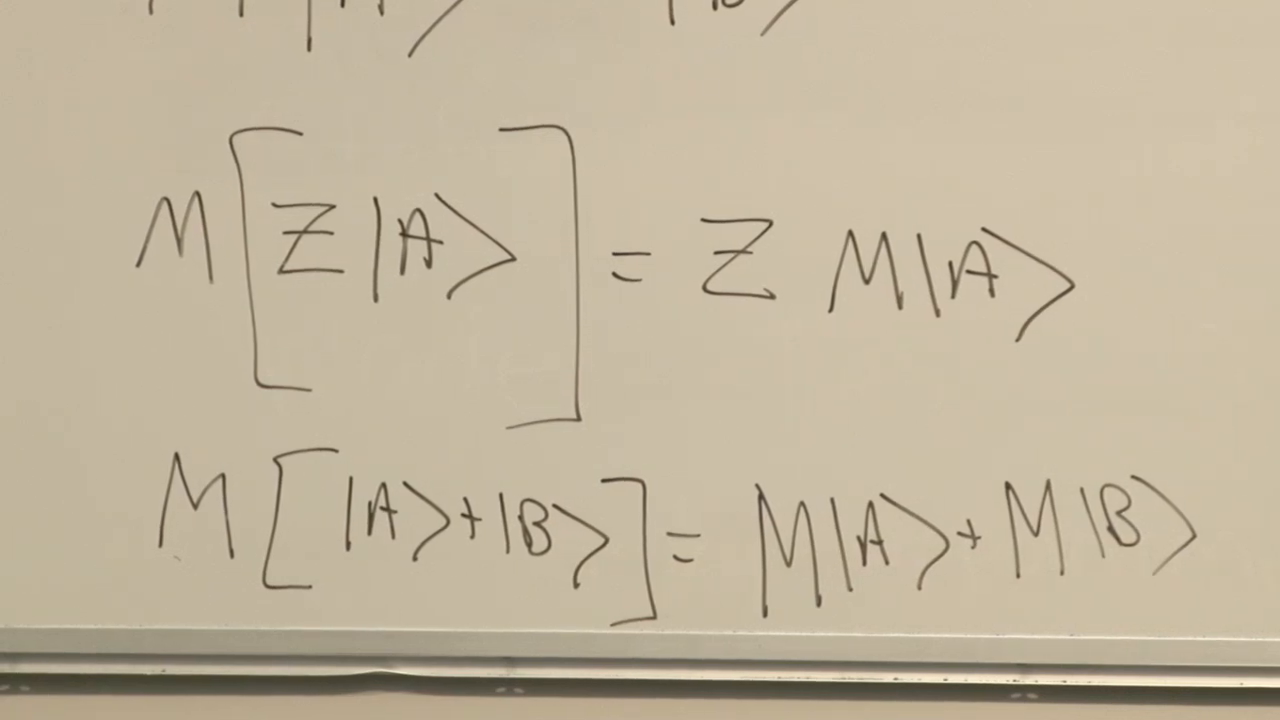
\includegraphics[width=0.82\textwidth]{lecture_03_figure_04.png}
\caption{基底の復習の後に書かれた、線形演算子の2つの定義規則。}
\lectureframe{00:12:44}
\end{figure}

\section{機械としての線形演算子}

線形演算子\(M\)は、入力ケットを一意の出力ケットに写す規則である。ジョン・ホイーラーによる有用な描像は、入力ポートと出力ポートをもつ機械である。\(\ket{A}\)を入れ、車輪を回すと\(M\ket{A}\)を受け取る。出力は入力によって定まる。逆は一意である必要はない。2つの入力が同じ出力を生むこともあり、逆機械が存在する必要もない。

\emph{線形}という形容詞は2つの規則からなる。複素数\(z\)に対して、
\begin{align}
M\bigl(z\ket{A}\bigr)&=z\,M\ket{A}, \label{eq:operator-homogeneous}\\
M\bigl(\ket{A}+\ket{B}\bigr)&=M\ket{A}+M\ket{B}.
\label{eq:operator-additive}
\end{align}
スカラーは機械をそのまま通過し、和は1項ずつ処理できる。これらの規則は任意の有限複素線形結合に対する線形性も意味する。

同じ考え方は通常の3次元ベクトルにも当てはまる。量子力学は線形写像を発明したのではない。状態空間が抽象的で複素的であること、そして可測量がそのような写像の特別な族によって表されることから、それらを不可欠なものにしている。

\section{演算子からその行列へ}

機械が\(\ket{A}\)を\(\ket{B}\)に送るとする：
\begin{equation}
M\ket{A}=\ket{B}.
\label{eq:operator-action}
\end{equation}
入力と出力に同じ正規直交基底を選び、
\[
\ket{A}=\sum_j\alpha_j\ket{j},
\qquad
\ket{B}=\sum_i\beta_i\ket{i}.
\]
と書く。\(i\)番目の出力成分を求めるには、式~\eqref{eq:operator-action}を\(\bra{i}\)で射影する：
\begin{equation}
\bra{i}M\ket{A}=\braket{i}{B}=\beta_i.
\end{equation}
次に\(\ket{A}\)の展開を挿入する：
\begin{align}
\bra{i}M\ket{A}
 &=\sum_j\bra{i}M\ket{j}\braket{j}{A}\\
 &=\sum_j\bra{i}M\ket{j}\alpha_j
 =\beta_i.
\end{align}
数
\begin{equation}
m_{ij}\equiv\bra{i}M\ket{j}
\label{eq:matrix-elements}
\end{equation}
は、選んだ基底における\(M\)の\emph{行列要素}である。したがって、
\begin{equation}
\boxed{\sum_jm_{ij}\alpha_j=\beta_i.}
\label{eq:component-action}
\end{equation}

\begin{figure}[htbp]
\centering
\includegraphics[width=0.84\textwidth]{lecture_03_figure_02.png}
\caption{抽象的な式\(M\ket{A}=\ket{B}\)を射影し、成分規則\(\sum_jm_{ij}\alpha_j=\beta_i\)に分解したもの。}
\lectureframe{00:18:30}
\end{figure}

空間の次元が\(N\)なら、\(N^2\)個の数\(m_{ij}\)は\(N\times N\)正方行列をなす。式~\eqref{eq:component-action}はまさに
\begin{equation}
\begin{pmatrix}
m_{11}&m_{12}&\cdots&m_{1N}\\
m_{21}&m_{22}&\cdots&m_{2N}\\
\vdots&\vdots&\ddots&\vdots\\
m_{N1}&m_{N2}&\cdots&m_{NN}
\end{pmatrix}
\begin{pmatrix}
\alpha_1\\
\alpha_2\\
\vdots\\
\alpha_N
\end{pmatrix}
=
\begin{pmatrix}
\beta_1\\
\beta_2\\
\vdots\\
\beta_N
\end{pmatrix}.
\label{eq:matrix-vector-action}
\end{equation}
である。\(\beta_1\)を得るには、第1行を入力列に掛けて加える。\(\beta_2\)についても第2行で繰り返し、以下同様にする。行列はホイーラーの機械の具体的な姿である。

\begin{figure}[htbp]
\centering
\includegraphics[width=0.84\textwidth]{lecture_03_figure_03.png}
\caption{同じ演算子の作用を、入力係数列に掛ける正方行列として表示したもの。}
\lectureframe{00:20:01}
\end{figure}

我々はアルゴリズムを得て、目に見える幾何学の一部を失った。抽象的な命題\(M\ket{A}=\ket{B}\)は座標に依存しない。個々の成分\(m_{ij}\)、\(\alpha_j\)、\(\beta_i\)は選択した基底に依存する。異なる正規直交基底は三つの配列すべてを変えるが、その下にある写像とその物理的予言は変えない。

\begin{classroomqa}
\audiencequestion{基底の選択は問題が解けるかどうかを決められるか。}
\lecturerresponse{解が容易に見えるかどうかは決められる。よく選ばれた基底は演算子を対角化し、計算をほとんど即座にできるかもしれない。悪い基底は構造を不快な代数の下に隠すかもしれない。実験の結果を変えることはできない。二つの基底が異なる物理的答えを導くなら、その計算は間違っている。}
\end{classroomqa}

\section{ブラ、ケット、反線形性}

\begin{classroomqa}
\audiencequestion{線形演算子はケットをブラに、またはブラをケットに変えられるか。}
\lecturerresponse{今定義した種類の通常の線形演算子ではない。それはケットをケットに写し、複素スカラーはそのまま通過する。ケットとブラを交換する操作はその係数を複素共役にするので、別のクラスに属する。}
\end{classroomqa}

固定された複素数による乗算は単純な線形演算子である。複素共役はそうではない。\(K\)が共役を表すなら、
\[
K\bigl(z\ket{A}\bigr)=z^*K\ket{A},
\]
であり、\(zK\ket{A}\)ではない。このような写像は\emph{反線形}と呼ばれる。この名前は線形の反対を意味しない。スカラーの共役を記録するものである。反粒子とのより深い関係は現在の議論の範囲を超えている。

それでも線形演算子をブラに作用させることができる。慣例により演算子は右側に書かれる：
\begin{equation}
\bra{A}M.
\end{equation}
定義は行列要素に括弧の曖昧さがないように選ばれている：
\begin{equation}
\bra{A}\bigl(M\ket{B}\bigr)
=
\bigl(\bra{A}M\bigr)\ket{B}
\equiv
\bra{A}M\ket{B}.
\label{eq:bracket-independence}
\end{equation}

なぜこれが可能かを見るために、両方のベクトルを展開する：
\begin{align}
\bra{A}M\ket{B}
 &=\left(\sum_i\alpha_i^*\bra{i}\right)
   M
   \left(\sum_j\beta_j\ket{j}\right)\\
 &=\sum_{ij}\alpha_i^*m_{ij}\beta_j.
\label{eq:matrix-element-double-sum}
\end{align}
これは通常の二重和である。\(j\)について先に和を取り、\(M\)がケットに作用すると見なしてもよいし、\(i\)について先に和を取り、それがブラに作用すると見なしてもよい。答えは同じである。記法は不要な括弧を除去できるようにまさにこのように整えられている。

\section{ダガー操作}

ブラ側には第二の異なる問いがある。次を仮定する：
\[
M\ket{A}=\ket{B}.
\]
対応するブラ\(\bra{A}\)を\(\bra{B}\)に変える演算子は何か。一般には\(M\)自身ではない。もし\(M\)が複素数\(z\)による乗算なら、ケット方程式は\(\ket{B}=z\ket{A}\)であり、ブラ方程式は\(\bra{B}=z^*\bra{A}\)であろう。

必要な演算子は\(M^\dagger\)、すなわち\(M\)の\emph{エルミート共役}と表記され、次で定義される：
\begin{equation}
M\ket{A}=\ket{B}
\quad\Longleftrightarrow\quad
\bra{A}M^\dagger=\bra{B}.
\label{eq:dagger-definition}
\end{equation}
ダガーは複素共役の演算子版である。

その行列規則は直接に従う。次を置く：
\[
M\ket{i}=\ket{i'}.
\]
すると
\[
m_{ji}=\bra{j}M\ket{i}=\braket{j}{i'}.
\]
ダガー化されたブラ関係は\(\bra{i}M^\dagger=\bra{i'}\)なので、
\[
(m^\dagger)_{ij}
=\bra{i}M^\dagger\ket{j}
=\braket{i'}{j}.
\]
内積を逆にすると複素共役になる：
\[
\braket{i'}{j}=\braket{j}{i'}^*.
\]
したがって
\begin{equation}
\boxed{(m^\dagger)_{ij}=m_{ji}^*.}
\label{eq:dagger-matrix-elements}
\end{equation}

\begin{figure}[htbp]
\centering
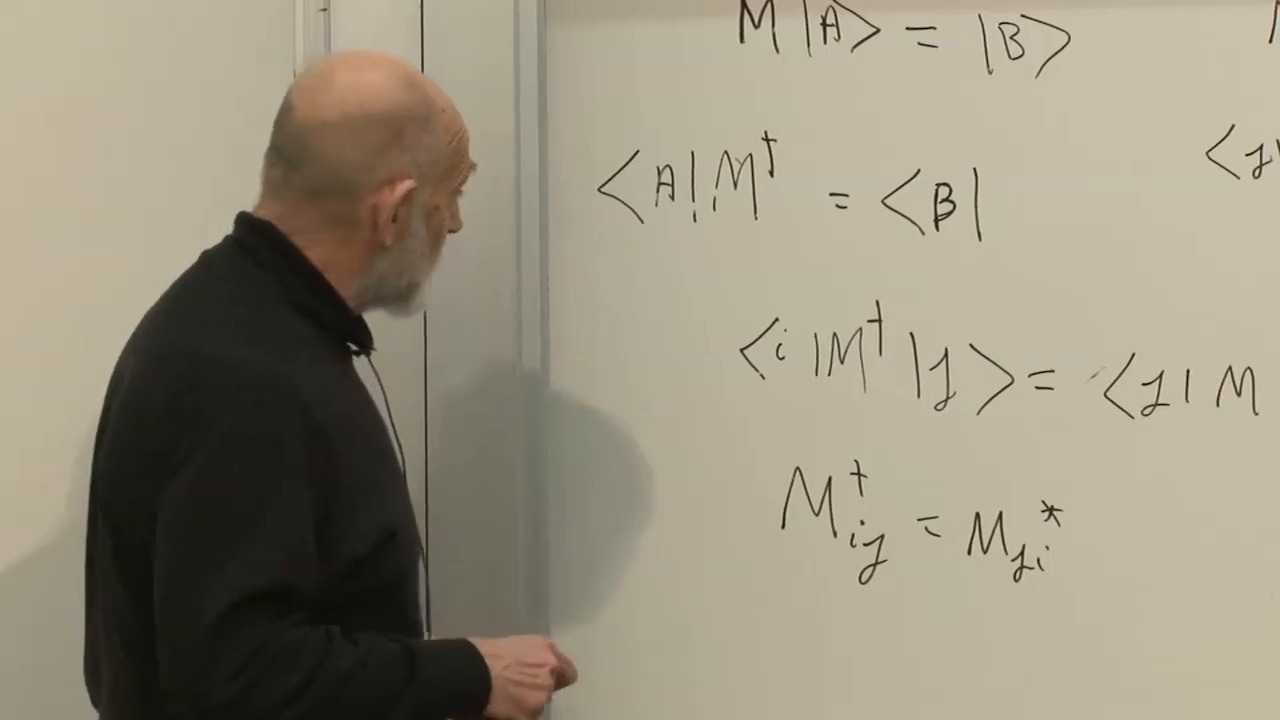
\includegraphics[width=0.84\textwidth]{lecture_03_figure_05.png}
\caption{エルミート共役の完成した黒板関係：添字を交換し複素共役を取る。}
\lectureframe{00:42:23}
\end{figure}

行列の言葉では転置してから複素共役を取る：
\begin{equation}
\begin{pmatrix}
a&b\\
c&d
\end{pmatrix}^{\!\dagger}
=
\begin{pmatrix}
a^*&c^*\\
b^*&d^*
\end{pmatrix}.
\label{eq:dagger-two-by-two}
\end{equation}
転置は主対角線を挟んで成分を反映する。共役はすべての\(i\)を\(-i\)に置き換える。例えば、
\begin{equation}
\begin{pmatrix}
2&6+7i\\
4-i&9+i
\end{pmatrix}^{\!\dagger}
=
\begin{pmatrix}
2&4+i\\
6-7i&9-i
\end{pmatrix}.
\label{eq:dagger-numerical-example}
\end{equation}
対角成分は位置を保つが共役化され、二つの非対角成分は位置を交換し共役化される。

\section{エルミート演算子}

複素数が実数であるのは、それ自身の複素共役に等しいまさにそのときである。演算子版は即座である。

\begin{definition}
演算子\(M\)は次を満たすとき\emph{エルミート}である：
\begin{equation}
M=M^\dagger.
\label{eq:hermitian-definition}
\end{equation}
同値に、すべての正規直交基底で、
\begin{equation}
m_{ij}=m_{ji}^*.
\label{eq:hermitian-components}
\end{equation}
\end{definition}

式~\eqref{eq:hermitian-components}で\(i=j\)と置く。すると
\[
m_{ii}=m_{ii}^*,
\]
なのですべての対角成分は実数である。対角線から離れて、成分は共役反射対で現れる。一つの成分が\(4-i\)なら、その反射相手は\(4+i\)である。一つが実数\(5\)なら、その相手もそうである。

\begin{figure}[htbp]
\centering
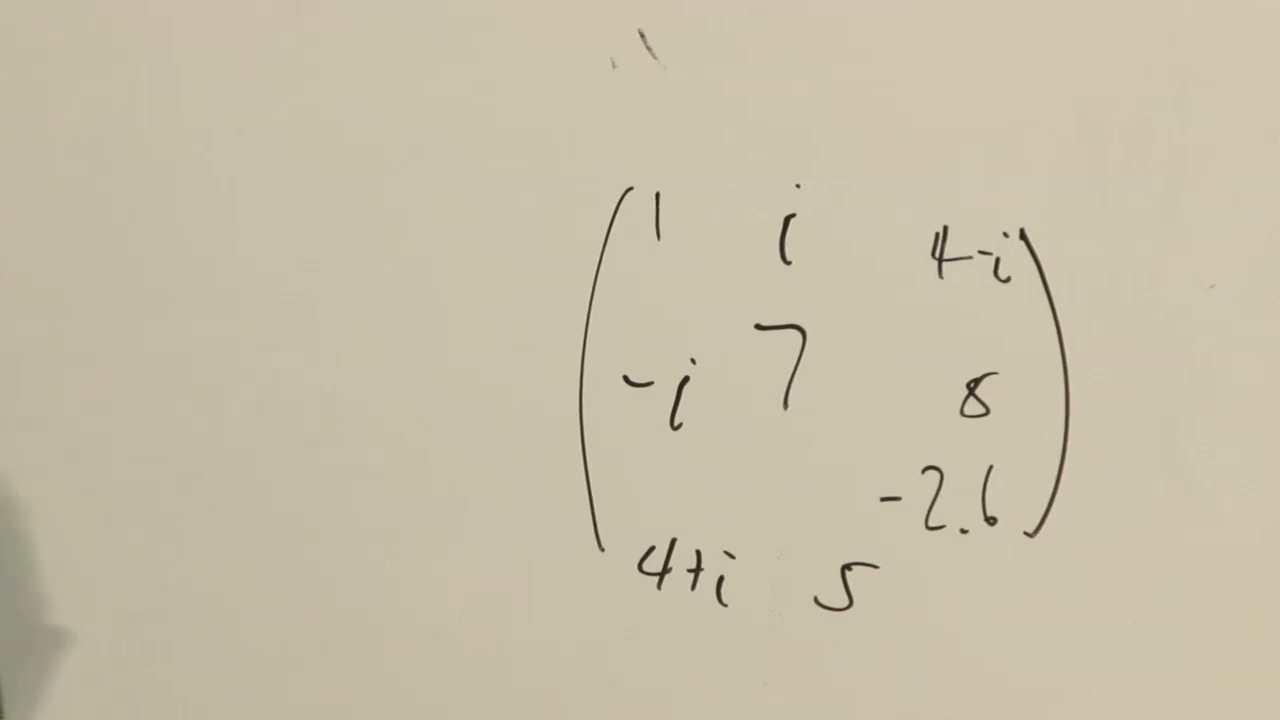
\includegraphics[width=0.78\textwidth]{lecture_03_figure_06.png}
\caption{完成したエルミート行列の例：対角線上に実数成分、それを挟んで反射された複素共役対。}
\lectureframe{00:45:43}
\end{figure}

エルミート演算子は測定可能な量を表すことになるので重要である。その同定を行う前に、それらの固有方向を理解する必要がある。

\section{固有ベクトルと固有方向}

固有ベクトルとの最初の出会いは、この部分を周囲の物理学より速く感じさせるかもしれない。その考えは新しい物理的仮説ではなく標準的な線形代数である。もし馴染みがなければ、定義を静かに復習してから議論に戻る価値がある。

一般の演算子はベクトルの向きを変える。例えば通常の三次元空間における回転は、ほとんどすべてのベクトルをそれ自身から離れた向きへと回す。回転軸は例外的である。その軸に沿ったベクトルは同じ向きのまま戻ってくる。これが固有ベクトルの模型である。

実二次元平面の非自明な回転は、反対の可能性を例示している。すなわち、実スケールを除いて固定される実の向きは存在しない。したがって、制限された実空間上の一般の演算子が実の固有ベクトルをもつ必要はない。量子力学で用いられる複素状態空間上のエルミート演算子は、はるかに強い性質をもつ。

\(M\)の固有ベクトルは
\begin{equation}
M\ket{i}=\lambda_i\ket{i}.
\label{eq:eigenvalue-equation}
\end{equation}
を満たす。数\(\lambda_i\)がその固有値である。固有ベクトルは演算子に属する。どの写像がその向きを保つのかを指定せずに固有ベクトルについて語ることはない。

その長さと位相は式~\eqref{eq:eigenvalue-equation}によって固定されない。すべての非零複素数\(z\)に対して、
\[
M\bigl(z\ket{i}\bigr)
=zM\ket{i}
=\lambda_i\bigl(z\ket{i}\bigr).
\]
したがって、\emph{固有方向}について語るほうがより正確である。\(\ket{i}\)のすべての非零倍は同じ向きを表し、同じ固有値をもつ。通常は規格化された代表元を選ぶ。

中心となるスペクトル的事実は次のとおりである。\(N\)次元複素ベクトル空間上のエルミート演算子は、\(N\)個の固有ベクトルからなる完全な正規直交基底をもつ。この主張のうち二つの部分は、ごくわずかな代数で確かめられる。

\subsection{エルミート演算子の固有値は実である}

\(M=M^\dagger\)かつ
\[
M\ket{i}=\lambda_i\ket{i}.
\]
を仮定する。方程式全体のエルミート共役をとると、
\begin{equation}
\bra{i}M^\dagger=\lambda_i^*\bra{i}.
\label{eq:eigen-bra-equation}
\end{equation}
\(M^\dagger=M\)であるから、ケット方程式に\(\bra{i}\)を掛け、ブラ方程式に\(\ket{i}\)を掛けると、
\begin{align}
\bra{i}M\ket{i}&=\lambda_i\braket{i}{i},\\
\bra{i}M\ket{i}&=\lambda_i^*\braket{i}{i}.
\end{align}
同じ非零のノルムが両方の数に掛かるので、
\begin{equation}
\lambda_i=\lambda_i^*.
\end{equation}
エルミート演算子のすべての固有値は実である。これは、そのような演算子が測定装置によって表示される実数を表しうることの最初の手がかりである。

\subsection{異なる固有値は直交する固有ベクトルを与える}


\[
M\ket{i}=\lambda_i\ket{i},
\qquad
M\ket{j}=\lambda_j\ket{j},
\]
とする。ここで\(M\)はエルミートである。第二の方程式のダガーをとる。その固有値はすでに実であることが知られている。
\[
\bra{j}M=\lambda_j\bra{j}.
\]
次に、第一の方程式に\(\bra{j}\)を掛け、ブラ方程式に\(\ket{i}\)を掛けると、
\begin{align}
\bra{j}M\ket{i}&=\lambda_i\braket{j}{i},\\
\bra{j}M\ket{i}&=\lambda_j\braket{j}{i}.
\end{align}
差をとると、
\begin{equation}
\boxed{(\lambda_i-\lambda_j)\braket{j}{i}=0.}
\label{eq:hermitian-orthogonality}
\end{equation}
\(\lambda_i\ne\lambda_j\)ならば、
\[
\braket{j}{i}=0.
\]
固有方向は直交する。

\begin{figure}[htbp]
\centering
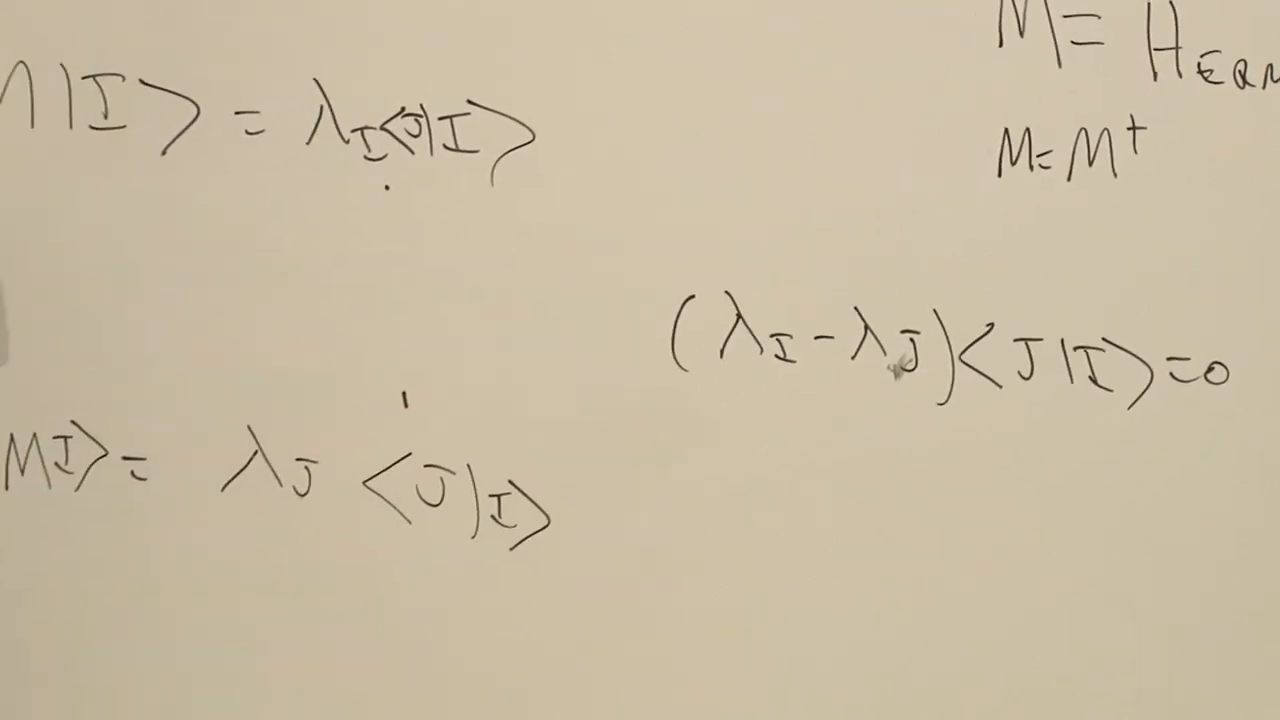
\includegraphics[width=0.82\textwidth]{lecture_03_figure_07.png}
\caption{直交性の証明における決定的な行：等しくない固有値は内積を零にする。}
\lectureframe{00:59:00}
\end{figure}

二つの固有値がたまたま等しいとき、式~\eqref{eq:hermitian-orthogonality}はその縮退した固有空間の内部に何の条件も課さない。そこでは正規直交基底を選ぶことができる。残りの固有方向と合わせて、それらのベクトルはスペクトル定理が約束する完全な正規直交固有基底をなす。

直交性には物理的な読み方もある。二つの直交する状態は、適切な測定によって曖昧さなく区別できる。異なる固有値をもつ固有状態は、装置がそれらに対して異なる実数を報告するのだから、区別可能でなければならない。代数と操作的意味はすでに同じ対応を指し示している。

\section{測定の公準}

これで、基本的な量子力学の対応を述べるのに十分な形式主義がそろった。初めて出会うときには異質に聞こえるかもしれない。その意味は使われて初めて具体的になるので、ここではそれらを簡潔に述べ、すぐにスピン実験へ戻ることにしよう。

一回の測定は一つの実数を生み出す。二つの両立する実数の読みを一つの複素数にまとめることはできるが、そのまとまりは依然として二つの測定を含んでいる。一つの検出器の素的な出力は実である。したがってエルミート演算子が自然な候補となる。その固有値は実であり、その固有ベクトルは完全な正規直交基底をなす。

\begin{enumerate}
\item 測定可能な量、すなわち\emph{可観測量}は、エルミート演算子\(M\)によって表される。
\item \(M\)を測定したときの可能な結果は、その固有値\(\lambda_i\)である。
\item \(M\)が確定値\(\lambda_i\)をもつ状態は、
\[
M\ket{i}=\lambda_i\ket{i}.
\]
を満たす固有状態\(\ket{i}\)である。
\item 系が一般の規格化された状態\(\ket{A}\)にあるならば、\(\lambda_i\)を得る確率は
\begin{equation}
P(\lambda_i\mid A)
=\left|\braket{i}{A}\right|^2
=\braket{i}{A}\braket{A}{i}.
\label{eq:born-rule}
\end{equation}
\end{enumerate}

この一覧は便利な出発点であり、必ずしも最小の独立な公理系ではない。より経済的な定式化では、いくつかの主張を他のものから導くことができる。対応を別々に保つことで、それらの物理的役割が見やすくなる。

複素数 \(\braket{i}{A}\) は \emph{確率振幅} であり、確率ではない。その複素共役を掛けると実数の非負の数が得られる。スピン成分の場合、スペクトルは \(+1\) と \(-1\) の二つの値しか持たないが、より一般的な観測量は多くの固有値を持ちうる。

\begin{figure}[htbp]
\centering
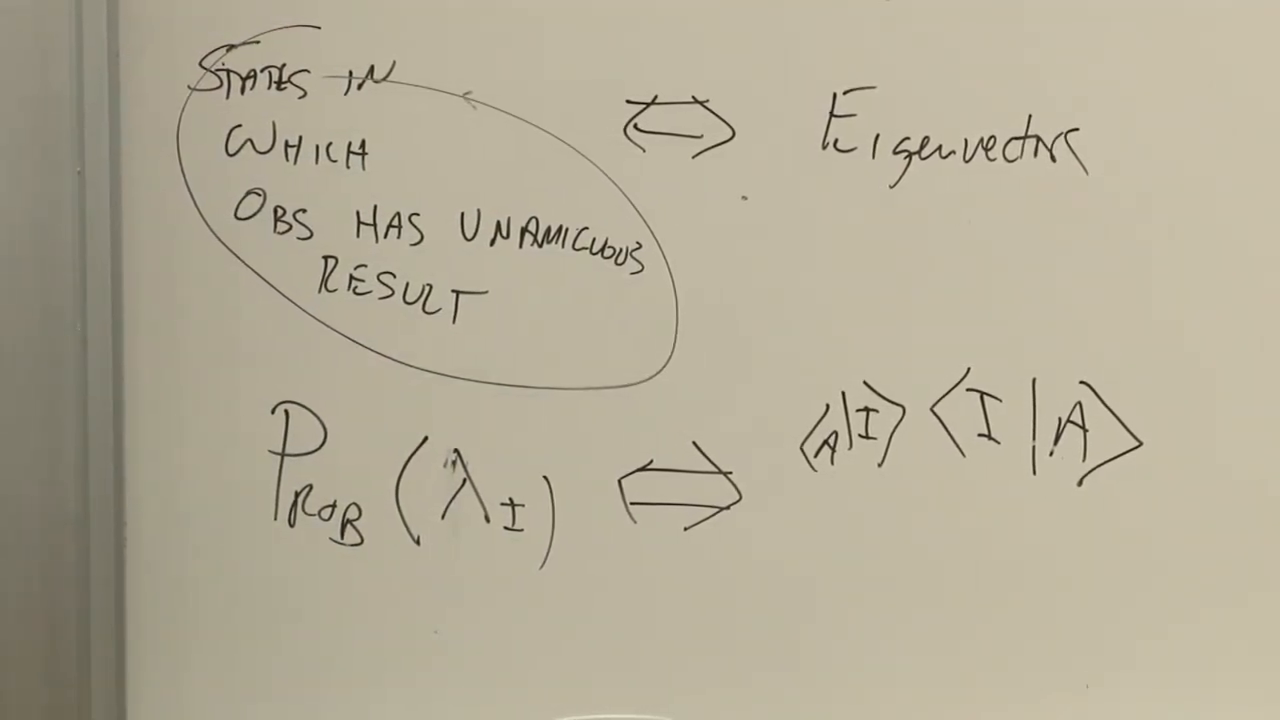
\includegraphics[width=0.82\textwidth]{lecture_03_figure_08.png}
\caption{この板書は、確定した結果を持つ状態を固有ベクトルと結び付け、\(\lambda_i\) の確率を \(\ket{i}\) への射影の絶対値の二乗と結び付けている。}
\lectureframe{01:11:29}
\end{figure}

\begin{classroomqa}
\audiencequestion{確率規則において \(P\) の隣に正確に何が書かれているか。}
\lecturerresponse{それは \(\lambda_i\) である。\(P(\lambda_i\mid A)\) は、系が \(\ket{A}\) に準備されているとき、\(M\) の測定が特定の固有値 \(\lambda_i\) を返す確率を意味する。右辺はその固有ベクトルへの射影の絶対値の二乗である。}
\end{classroomqa}

\subsection{規格化と完全性}

互いに排他的なすべての結果の確率の和は 1 でなければならない：
\begin{equation}
\sum_i\left|\braket{i}{A}\right|^2=1.
\label{eq:probability-normalization}
\end{equation}
完全な固有基底を挿入すると：
\begin{align}
\sum_i\left|\braket{i}{A}\right|^2
 &=\sum_i\braket{A}{i}\braket{i}{A}\\
 &=\bra{A}\left(\sum_i\ket{i}\bra{i}\right)\ket{A}\\
 &=\braket{A}{A}.
\end{align}
したがって、許される状態ベクトルは規格化されており、
\begin{equation}
\braket{A}{A}=1.
\label{eq:state-normalization}
\end{equation}
\(\ket{A}=\sum_i\alpha_i\ket{i}\) ならば、同じ条件は
\begin{equation}
\sum_i\alpha_i^*\alpha_i=1.
\label{eq:component-normalization}
\end{equation}
となる。これは複素成分に対する一つの実の拘束条件である。

\begin{classroomqa}
\audiencequestion{すべての確率は正でなければならないか。}
\lecturerresponse{はい。各確率はある数とその複素共役の積であるから、非負である。すると規格化により、そのようなすべての数の和が 1 に等しくなる。}
\end{classroomqa}

もう一つの冗長性がある。すべての成分に同じ位相を掛けると、
\begin{equation}
\ket{A}\longmapsto e^{i\theta}\ket{A},
\label{eq:l3-global-phase}
\end{equation}
すべての振幅が \(e^{i\theta}\) 倍され、すべての絶対値の二乗は変わらない。どの測定もその共通位相を検出できない。成分間の相対位相は物理的であり続ける。状態全体に掛かる位相だけが冗長である。

したがって、任意の複素ベクトルにおける二つの実パラメータは物理状態を指定しない。その大きさは規格化によって固定され、その全体位相は観測不能である。これは単一のスピンについて遭遇したのと同じパラメータ数であり、今や一般の確率規則から導かれたものである。

\subsection{測定は状態も準備する}

さらにもう一つの公理は、短い黒板の一行に圧縮するよりも口で言う方が容易である。測定が \(\lambda_i\) を返すならば、その直後に系は対応する固有状態 \(\ket{i}\) にある。装置は結果を記録すると同時に、同じ測定を繰り返せばその確定した結果が得られるような状態を準備する。

\begin{classroomqa}
\audiencequestion{その測定による準備の記述をもう一度言えるか。}
\lecturerresponse{測定の前には、式~\eqref{eq:born-rule}の確率でいくつかの固有値が生じうる。装置が実際に \(\lambda_i\) を報告すると、系は \(\lambda_i\) に属する固有状態に残される。したがって、同じ観測量を直ちにもう一度測定すると同じ値が返る。}
\end{classroomqa}

\begin{classroomqa}
\audiencequestion{これらの原理はすでに状態が時間とともにどのように発展するかを教えているか。}
\lecturerresponse{まだである。我々は状態とは何か、観測量がどのように表現されるか、測定が何をするかを指定した。時間に伴う変化を支配する法則は追加の構造であり、後に導入される。これは、運動方程式を書く前にまず古典的位相空間を定義するのに類似している。}
\end{classroomqa}

\begin{classroomqa}
\audiencequestion{以前、傾いた軸に沿った平均スピンには \(\cos\theta\) が現れた。新しい絶対値の二乗の規則はそれを \(\cos^2\theta\) にすべきか。}
\lecturerresponse{確率と平均は異なる量である。平均は \(+1\) と \(-1\) の結果の確率をそれらの符号とともに組み合わせる。任意方向のスピノルを構成すれば、絶対値の二乗の振幅は以前の余弦の平均を再現する。その計算は次の応用であり、古い式を変えて推測すべきものではない。}
\end{classroomqa}

\section{最初の応用としてのスピン}

三つの測定可能なスピン成分はエルミート演算子で表される：
\[
\sigma_x,\qquad \sigma_y,\qquad \sigma_z.
\]
分析器の実験はすでにそれらの可能な値と確定値状態を与えていた：
\[
\begin{array}{c|c|c}
\text{observable}&\text{eigenvalue }+1&\text{eigenvalue }-1\\ \hline
\sigma_z&\ket{u}&\ket{d}\\
\sigma_x&\ket{r}&\ket{l}\\
\sigma_y&\ket{\mathrm{in}}&\ket{\mathrm{out}}
\end{array}
\]
この情報で演算子を行列として再構成するのに十分である。

\subsection{固有基底における z 成分}

アップ--ダウン基底を選ぶ。確定した \(z\) スピンは
\begin{equation}
\sigma_z\ket{u}=+\ket{u},
\qquad
\sigma_z\ket{d}=-\ket{d}.
\label{eq:sigma-z-eigenvectors}
\end{equation}
を意味する。二つの固有値は異なるので、エルミート性は \(\braket{u}{d}=0\) を意味する。

四つの行列要素を計算する：
\begin{align}
\bra{u}\sigma_z\ket{u}&=+1,&
\bra{u}\sigma_z\ket{d}&=-\braket{u}{d}=0,\\
\bra{d}\sigma_z\ket{u}&=\braket{d}{u}=0,&
\bra{d}\sigma_z\ket{d}&=-1.
\end{align}
したがって
\begin{equation}
\boxed{
\sigma_z=
\begin{pmatrix}
1&0\\
0&-1
\end{pmatrix}_{\{u,d\}}.}
\label{eq:sigma-z}
\end{equation}
座標列は
\[
\ket{u}\widehat{=}\begin{pmatrix}1\\0\end{pmatrix},
\qquad
\ket{d}\widehat{=}\begin{pmatrix}0\\1\end{pmatrix}.
\]
式~\eqref{eq:sigma-z}を掛けると、第一列はそのまま返り、第二列は負符号付きで返る。まさに固有値方程式が要求する通りである。

\begin{figure}[htbp]
\centering
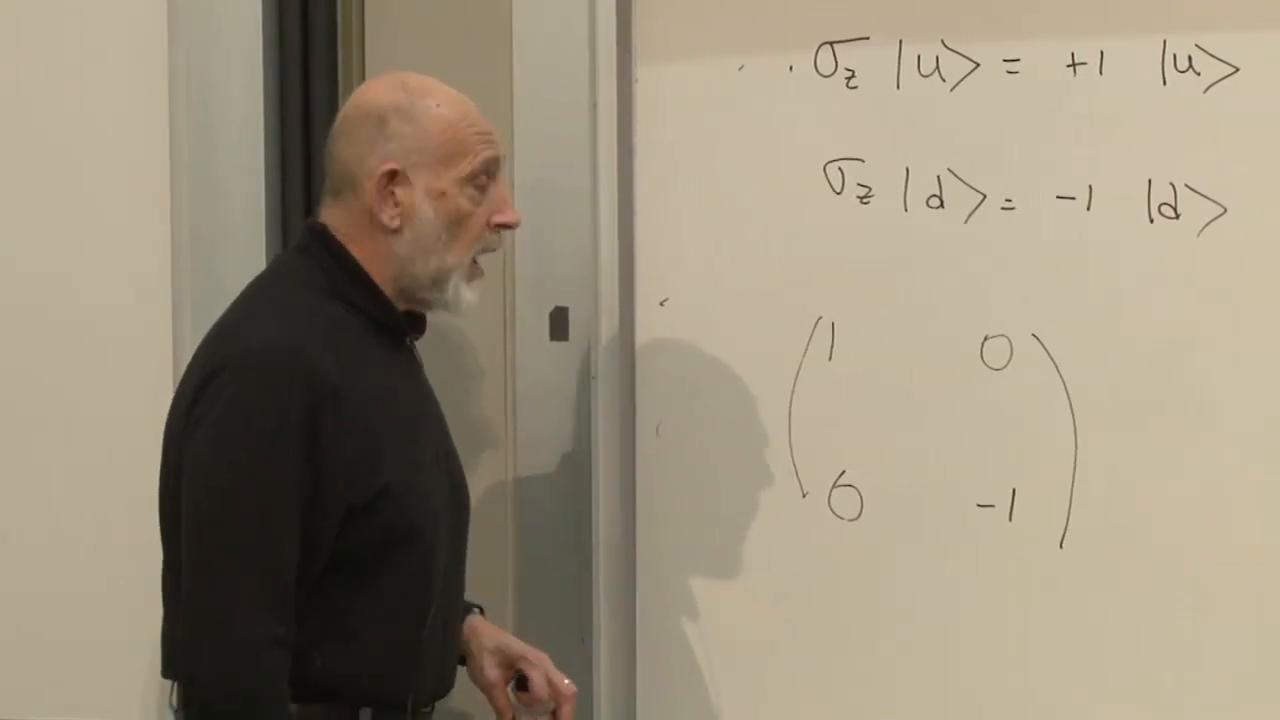
\includegraphics[width=0.82\textwidth]{lecture_03_figure_09.png}
\caption{上--下基底における\(\sigma_z\)の固有値方程式と、その結果得られる対角行列。}
\lectureframe{01:26:56}
\end{figure}

\subsection{基底を変えずにx成分を求める}

右--左基底では、\(\sigma_x\)も同じ対角形になるであろう。それは容易であるが、情報量はない。上--下基底を保ち、
\begin{equation}
\sigma_x\ket{r}=+\ket{r},
\qquad
\sigma_x\ket{l}=-\ket{l}.
\label{eq:sigma-x-eigenvectors}
\end{equation}
を用いる。二つの基底は
\begin{align}
\ket{r}&=\frac{\ket{u}+\ket{d}}{\sqrt2},&
\ket{l}&=\frac{\ket{u}-\ket{d}}{\sqrt2},\\
\ket{u}&=\frac{\ket{r}+\ket{l}}{\sqrt2},&
\ket{d}&=\frac{\ket{r}-\ket{l}}{\sqrt2}.
\label{eq:x-z-basis-relations}
\end{align}
によって関係づけられる。

まず上側の対角成分から始める。
\begin{align}
\bra{u}\sigma_x\ket{u}
 &=\frac12(\bra{r}+\bra{l})\sigma_x(\ket{r}+\ket{l})\\
 &=\frac12(\bra{r}+\bra{l})(\ket{r}-\ket{l})\\
 &=0.
\end{align}
右状態と左状態は正規直交であるから、二つの対角項は相殺し、交差項は消える。\(\ket{d}\)について同じ計算を行うと
\[
\bra{d}\sigma_x\ket{d}=0.
\]
が得られる。この時点で二つのゼロは演算子が消えることを意味しない。それらは非対角成分を見よと告げているのである。

右上の成分については、
\begin{align}
\bra{u}\sigma_x\ket{d}
 &=\frac12(\bra{r}+\bra{l})\sigma_x(\ket{r}-\ket{l})\\
 &=\frac12(\bra{r}+\bra{l})(\ket{r}+\ket{l})\\
 &=1.
\end{align}
エルミート性、あるいは計算の直接の繰り返しにより、
\[
\bra{d}\sigma_x\ket{u}=1.
\]
が得られる。したがって
\begin{equation}
\boxed{
\sigma_x=
\begin{pmatrix}
0&1\\
1&0
\end{pmatrix}_{\{u,d\}}.}
\label{eq:sigma-x}
\end{equation}
同じ抽象演算子が、それ自身の固有基底では対角であり、\(z\)基底では非対角である。これは物理的曖昧さを伴わない基底依存性の具体的な一例である。

\subsection{y成分と相対位相}

規格化されたin--outの規約
\begin{equation}
\ket{\mathrm{in}}=\frac{\ket{u}+i\ket{d}}{\sqrt2},
\qquad
\ket{\mathrm{out}}=\frac{\ket{u}-i\ket{d}}{\sqrt2},
\label{eq:l3-in-out-states}
\end{equation}
を選ぶ。ここで
\[
\sigma_y\ket{\mathrm{in}}=+\ket{\mathrm{in}},
\qquad
\sigma_y\ket{\mathrm{out}}=-\ket{\mathrm{out}}.
\]
である。ラベルを入れ替えたり、\(y\)軸を反転させたりすることは、符号の規約を変えるだけで、根底にある構成を変えるものではない。式~\eqref{eq:l3-in-out-states}を用いると、これらの固有ベクトルと固有値をもつ唯一のエルミート行列は
\begin{equation}
\boxed{
\sigma_y=
\begin{pmatrix}
0&-i\\
i&0
\end{pmatrix}_{\{u,d\}}.}
\label{eq:sigma-y}
\end{equation}
である。再導出するよりも検証する方が容易である。
\begin{align}
\begin{pmatrix}0&-i\\i&0\end{pmatrix}
\frac1{\sqrt2}\begin{pmatrix}1\\i\end{pmatrix}
&=\frac1{\sqrt2}\begin{pmatrix}1\\i\end{pmatrix},\\
\begin{pmatrix}0&-i\\i&0\end{pmatrix}
\frac1{\sqrt2}\begin{pmatrix}1\\-i\end{pmatrix}
&=-\frac1{\sqrt2}\begin{pmatrix}1\\-i\end{pmatrix}.
\end{align}
\(1/\sqrt2\)の因子は固有ベクトルを規格化するが、それらの固有方向には影響しない。

\begin{figure}[htbp]
\centering
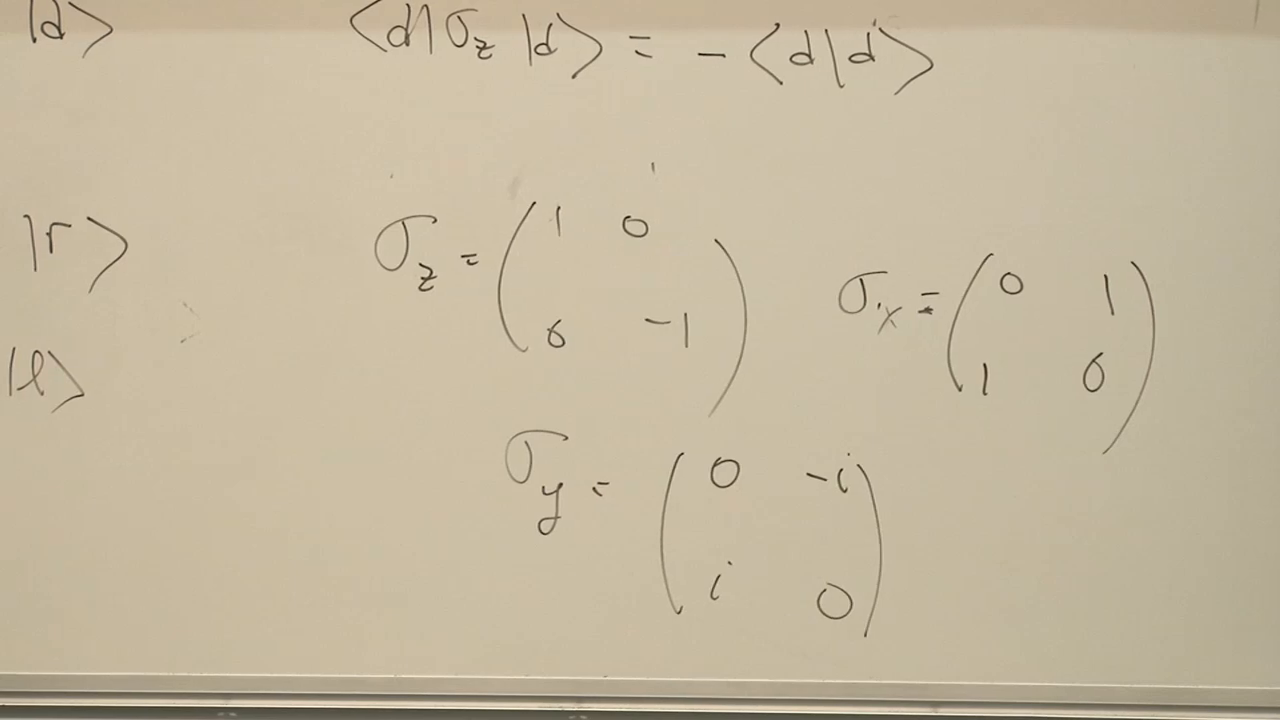
\includegraphics[width=0.82\textwidth]{lecture_03_figure_10.png}
\caption{上--下基底におけるパウリ行列の完成した板書一式。}
\lectureframe{01:38:11}
\end{figure}

\begin{classroomqa}
\audiencequestion{in--outベクトルを直交させるために、一方の符号を変えるべきでしょうか。}
\lecturerresponse{いいえ。欠けている手順は、ケットをブラに変える際の複素共役です。
\[
\bra{\mathrm{in}}=\frac{\bra{u}-i\bra{d}}{\sqrt2}.
\]
したがって
\[
\begin{aligned}
\braket{\mathrm{in}}{\mathrm{out}}
&=\frac12(\bra{u}-i\bra{d})
  (\ket{u}-i\ket{d})\\
&=\frac12\bigl(1+(-i)(-i)\bigr)\\
&=0.
\end{aligned}
\]
この共役を忘れることが、まさにブラ--ケット記法が明るみに出そうとしているよくある誤りです。}
\end{classroomqa}

我々は
\begin{equation}
\begin{aligned}
\sigma_x&=\begin{pmatrix}0&1\\1&0\end{pmatrix},\\[0.4em]
\sigma_y&=\begin{pmatrix}0&-i\\i&0\end{pmatrix},\\[0.4em]
\sigma_z&=\begin{pmatrix}1&0\\0&-1\end{pmatrix}.
\end{aligned}
\label{eq:pauli-triple}
\end{equation}
を得た。これらはエルミートであり、固有値\(\pm1\)をもち、分析器の実験が要求する確定スピンの固有ベクトルをまさに備えている。

次の問題は今や適切に定式化されている。任意の方向に準備されたスピンが与えられたとき、対応する状態を構成し、振幅の二乗を用いて\(\sigma_z=+1\)および\(\sigma_z=-1\)の確率を計算する。形式論はすでに十分な情報を含んでいる。その計算を実行することが自然な次の一歩である。
